\documentclass[conference]{IEEEtran}
\usepackage{amssymb,amsmath,graphicx,float,array,theorem}
\usepackage[noadjust]{cite}

\newcommand\real{\mathbb{R}}

\newtheorem{theorem}{Theorem}
\theorembodyfont{\itshape}

\DeclareMathOperator{\inv}{inv}

\begin{document}

\title{Point Stabilization of Mobile Robots with Model Predictive Control}

\author{\authorblockN{Felipe K\"{u}hne, Walter Fetter Lages and Jo\~{a}o Manoel Gomes da Silva Jr.}
\authorblockA{Federal University of Rio Grande do Sul \\
Electrical Engineering Department \\
Av. Oswaldo Aranha, 103 \\
Porto Alegre, RS 90035-190 Brazil \\
Email: \{kuhne,fetter,jmgomes\}@eletro.ufrgs.br}}

\maketitle

\begin{abstract}
This paper presents an optimal control scheme for a wheeled mobile robot (WMR) with nonholonomic constraints. Due to Brockett's conditions, it is well known that a WMR with nonholonomic constraints can not be feedback stabilized at a given configuration through continuously differentiable, time-invariant control laws. By using model predictive control (MPC), a time-varying control law is naturally obtained. One of the main advantages of MPC is the ability to handle constraints (due to state or input limitations) in a straightforward way. Furthermore, the control law obtained is optimal in a way that the control inputs are the minimizers of an objective function. A disadvantage of MPC is the large computational cost required to solve {\em on-line} the optimization problem. The point stabilization problem for the kinematic model of a WMR is solved and some simulation results are shown.
\end{abstract}

\section{Introduction}
\label{sec:intro}

The field of mobile robot control has been the focus of active research in the past decades. Despite the apparent simplicity of the kinematic model of a Wheeled Mobile Robot (WMR), the existence of nonholonomic (non-integrable) constraints turns the design of stabilizing control laws for those systems into a challenge. Due to Brockett's conditions~\cite{brockett82}, a continuously differentiable, time-invariant, static state feedback control law cannot be used to stabilize a nonholonomic system at a given posture. To overcome these limitations most works use non-smooth and time-varying control laws~(see \cite{bloch89,samson91,canudas92,yamamoto94,murray97} and the references therein). Recent works dealing with robust and adaptive control of WMRs can be found in \cite{oya03,dixon04}.

In realistic implementations, traditional techniques for the control of nonholonomic mechanical systems, such as non-smooth and time-varying control laws, often do not present good results, due to the constraints on inputs or states that naturally arise. In general, the resulting closed-loop trajectory presents unnecessary oscilatory motions. Furthermore, tuning parameters are difficult to choose since these control laws are not intuitively obtained and coordinate transformations to {\em chained} or {\em power} forms~\cite{bloch89} are used.

In this paper we show that, by using Model Predictive Control (MPC), all these disadvantages can be overcome: a time-varying control law is implicitly obtained, thus dealing with Brockett's conditions; the system model does not need to be transformed to another coordinate basis; the tuning parameters are easy to deal with; an objective function is minimized, which makes the control law optimal according to the optimization criterions; constraints on state and control inputs can be considered in a straightforward way. For a WMR the latter is an important issue, since the position of the robot can be restricted to belong to a safe region of operation, and also the oscilatory motions can be reduced. By considering input constraints, control actions that respect actuators limits can be generated.

Model predictive control (MPC) is an optimal control strategy that uses the model of the system to obtain an optimal control sequence by minimizing an objective function. At each sampling interval, the model is used to predict the behavior of the system over a prediction horizon. Based on these predictions, an objective function is minimized with respect to the future sequence of inputs, thus requiring the solution of a constrained optimization problem for each sampling interval. Although prediction and optimization are performed over a future horizon, only the values of the inputs for the current sampling interval are used and the same procedure is repeated at the next sampling time. This mechanism is known as {\it moving} or {\it receding horizon} strategy, in reference to the way in which the time window shifts forward from one sampling time to the next one.

For complex, constrained, multivariable control problems, MPC has become an accepted standard in the process industries~\cite{bemporad02}. It is used in many cases, where plants being controlled are sufficiently {\em slow} to allow its implementation~\cite{mayne00}. However, for systems with fast and nonlinear dynamics, which is the case of mobile robots, the implementation of predictive controllers remains fundamentally limited in applicability, due to large amount of {\em on-line} computation required~\cite{cannon00}. However, with the development of increasingly faster processors and efficient numerical algorithms, the use of MPC in such demanding applications becomes possible. Although MPC is not a new control method, works dealing with MPC of WMRs are recent and sparse~\cite{ollero91,rico99,essen01}.

This paper is organized as follows: in the next section the kinematic model of the WMR and some important model properties are shown. The MPC algorithm is depicted in section~\ref{sec:mpc}. Simulation results in {\sc Matlab} are shown in section~\ref{sec:simulations} and section~\ref{sec:conclusions} the conclusions are pointed out.


\section{Kinematic Model of the WMR}
\label{sec:model}

A mobile robot made up of a rigid body and non deforming wheels is considered (see Fig.~\ref{fig:robot}). It is assumed that the vehicle moves on a plane without slipping, i.e., there is a pure rolling contact between the wheels and the ground. The kinematic model of the WMR then is given by~\cite{Campion:TRA-12-1}:

\begin{equation}\label{eqn:model}
	\left\{
		\begin{aligned}
			\dot x	  &= v\cos\theta \\
			\dot y	  &= v\sin\theta \\
			\dot \theta &= w
		\end{aligned}
	\right.
\end{equation}

\noindent or, in a more compact form as
\begin{equation}
\label{eqn:modelshort}
	\dot{\bf x} = f({\bf x}){\bf u},	
\end{equation}

\noindent where ${\bf x}\triangleq[x~~y~~\theta]^T$ describes the configuration (position and orientation) of the center of the axis of the wheels, $C$, with respect to a global inertial frame $\{O,X,Y\}$. ${\bf u}\triangleq[v~~w]^T$ is the control input, where $v$ and $w$ are the linear and the angular velocities, respectively.

\begin{figure}[htbp]
	\centering
	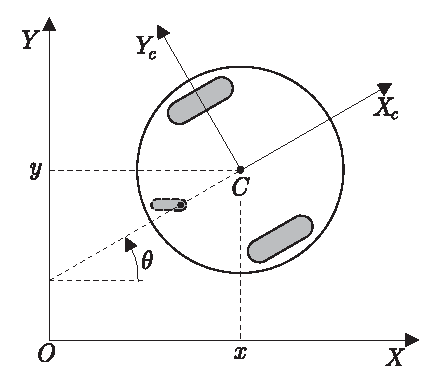
\includegraphics[width=0.67\linewidth]{Figures/robot.eps}
	\caption{Coordinate system of the WMR.}
	\label{fig:robot}
\end{figure}


\subsection{Model properties}
\label{sec:modelprop}

Although (\ref{eqn:model}) is a simplified model of the vehicles's motion (motor dynamics, elastic deformations and other mechanical effects are neglected), it is sufficient to capture the nonholonomy property which characterizes most mobile robots. Also, important properties regarding controllability and stabilizability of the WMR's can be shown, as pointed out in the following theorems.

\begin{theorem}[Controllability]\label{teo:cont}
A system is said to be controllable when it can be steered from any state configuration to any other in finite-time by using finite inputs~\cite{sontag90}. 

For driftless systems of the form

\begin{equation}
\label{eqn:driftless}
	\dot{\bf x} = \sum_{i=1}^{m}f_i({\bf x}){\bf u}_i \quad {\bf x}\in\real^n, {\bf u}\in\real^m
\end{equation}

\noindent a sufficient condition for controllability is that the dimension of the involutive closure of the distribution generated by the vector fields $f_i$ be equal to $n$, $\forall {\bf x}$, i.e.,
\begin{equation*}
	\dim\{\inv\Delta\}=n \qquad \Delta\triangleq span\{f_i\}
\end{equation*}

For the kinematic model~(\ref{eqn:model}), we have
\begin{equation*}
	rank\{f_1,f_2,[f_1,f_2]\} = rank\begin{bmatrix}
		\cos\theta & \sin\theta & 0 \\
		\sin\theta & -\cos\theta & 0 \\
		0 & 0 & 1 \end{bmatrix} = 3
\end{equation*}

Therefore, $\dim\{\inv\Delta\}=3$ and the system is controllable.
\end{theorem}

\begin{theorem}[Smooth static state-feedback stabilization]\label{teo:brockett}
The problem of smooth state feedback stabilization can be casted as to find a feedback control law ${\bf u}=k({\bf x})$ such that the closed-loop system $\dot{\bf x}=f({\bf x})k({\bf x})$ is asymptotically stable. 

Consider again the driftless system~(\ref{eqn:driftless}), with $m\leq n$. If the vectors $f_i(0)$ are linearly independent, i.e.,
\begin{equation*}
	rank[f_1(0)~~f_2(0)~~\cdots~~f_m(0)] = m,
\end{equation*}

\noindent then a solution to the above stabilization problem exists if and only if $m=n$.

\end{theorem}

Note that for the kinematic model~(\ref{eqn:model}), $n=3$ and $m=2$, therefore a smooth static state-feedback control law \mbox{${\bf u}=k({\bf x})$} does not exist for the considered WMR. Indeed, as opposed to linear systems, controllability of nonlinear systems does not imply the existence of stabilizing smooth static state feedbacks. Theorem~\ref{teo:brockett} is a corollary of the Brockett's conditions~\cite{brockett82}, particularized for the case of driftless systems.

\section{The MPC Algorithm}
\label{sec:mpc}

It was said in section~\ref{sec:intro} that the essence of a MPC scheme is to optimize predictions of process behavior over a sequence of future control inputs. Such a prediction is accomplished by using a process model over a finite time
interval, called the {\em prediction horizon}. At each sampling time, the model predictive controller generates an optimal control sequence by solving an optimization problem. The first element of this sequence is applied to the plant. The problem is solved again at the next sampling time using the updated process measurements and a shifted horizon. This scheme is described in Fig.~\ref{fig:mpc} below.

\begin{figure}[htbp]
	\centering
	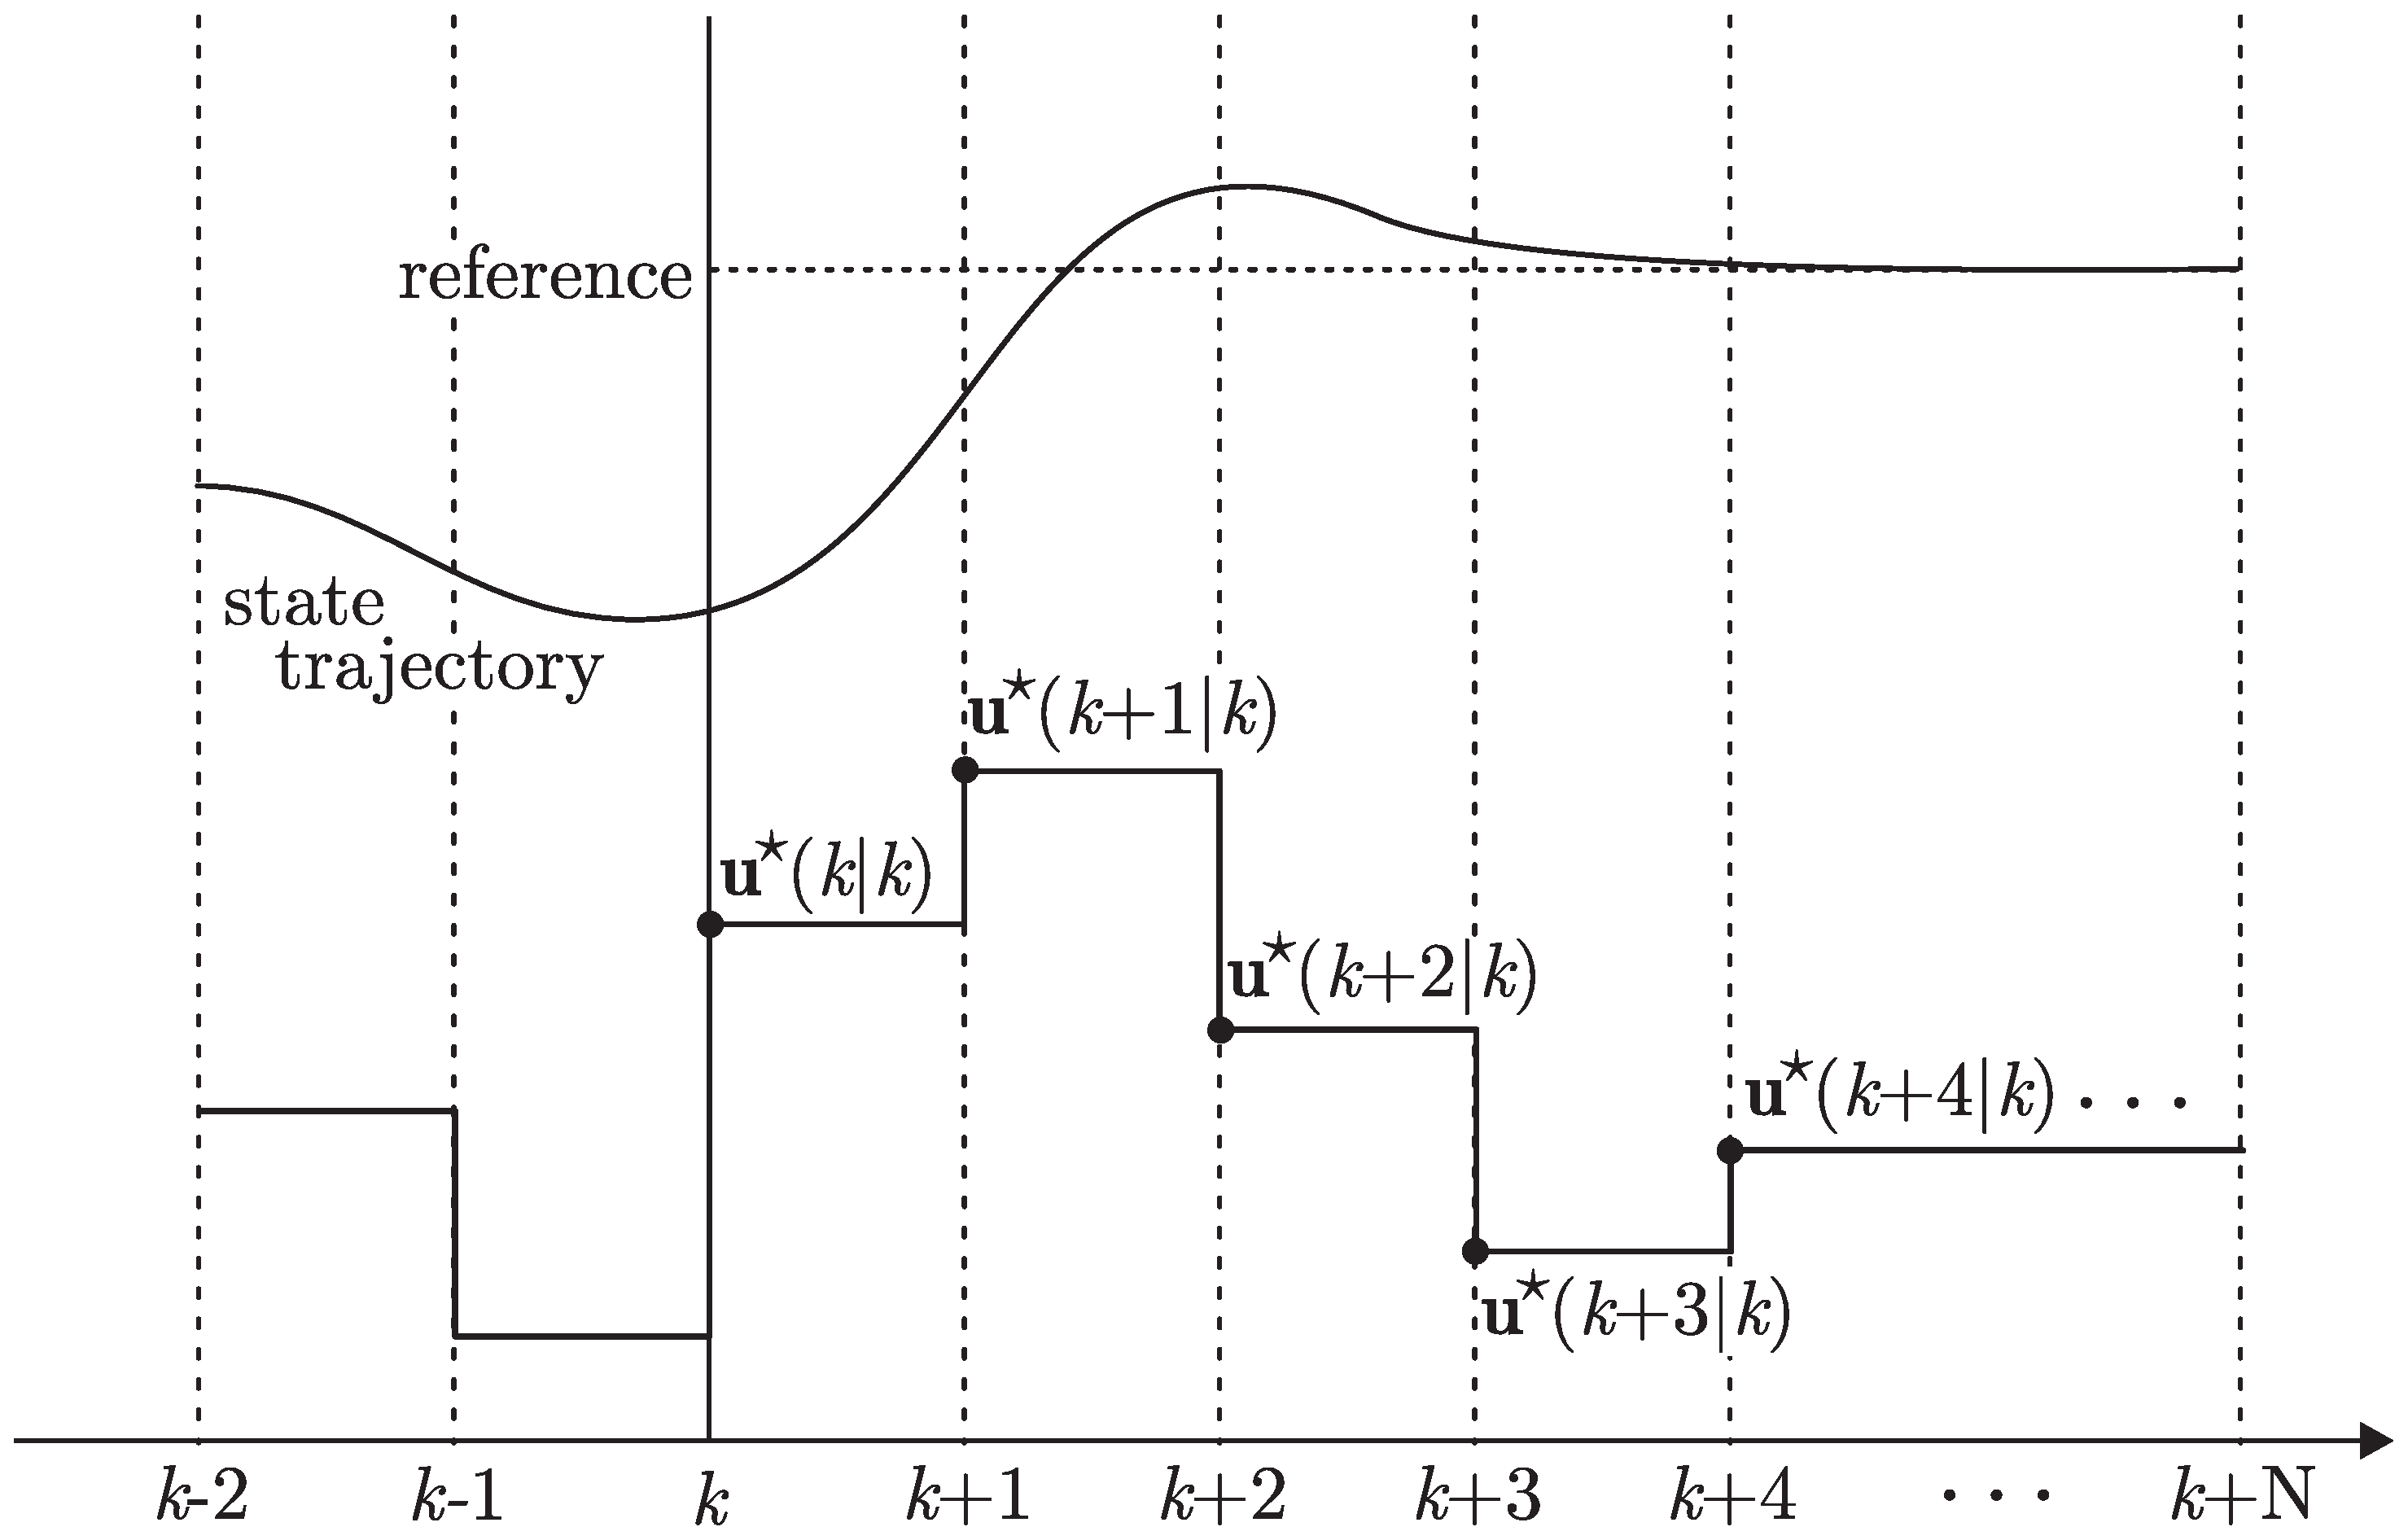
\includegraphics[width=\linewidth]{Figures/mpc3.eps}
	\caption{Model predictive control.}
	\label{fig:mpc}
\end{figure}

For the sake of simplicity, we assume in this work that the states of the plant are always available for measurement and that there are no plant/model mismatch.

The system model~(\ref{eqn:modelshort}) can be rewritten in discrete time, using forward differences and a sampling period os $T$ seconds:
\begin{equation*}
\label{eqn:discretemodelshort}
	{\bf x}(k+1) = f({\bf x}(k)){\bf u}(k),
\end{equation*}
where $k$ is the sampling time.

The objective function to be minimized can be stated as a quadratic function of the states and control inputs:

\begin{multline}
\label{eqn:cost}
	\Phi(k) = \sum_{j=1}^{N}{\bf x}^T(k+j|k){\bf Q}{\bf x}(k+j|k) + \\ + {\bf u}^T(k+j-1|k){\bf R}{\bf u}(k+j-1|k),
\end{multline}

\noindent where $N$ is the prediction horizon and ${\bf Q}$, ${\bf R}$ are weighting matrices used to penalize the state error and the control effort, respectively, with ${\bf Q}\geq 0$ and ${\bf R}>0$. The notation $a(m|n)$ indicates the value of $a$ at the instant $m$ predicted at instant $n$.

Hence, the optimization problem can be stated as to find ${\bf u}^\star$ such that:

\begin{equation}
\label{eqn:optim}
	{\bf u}^\star = \arg\min_{{\bf u}}\left\{\Phi(k)\right\}
\end{equation}
\noindent s. a.
\begin{align}
	{\bf x}(j+1) &= f({\bf x}(j)){\bf u}(j) \notag \\
	{\bf Cx}(j+1) &\leq {\bf c} \label{eqn:restx} \\
	{\bf Du}(j) &\leq {\bf d} \label{eqn:restu}
%	{\bf u}(j) &\in \mathbb{U} \label{eqn:restu} \\
%	{\bf x}(j) &\in \mathbb{X} \label{eqn:restx}	
\end{align}

\noindent where $j\in[k,k+N-1]$, $\Phi(k)$ is the objective function and ${\bf u}$ is the free variable in the optimization. 

The problem of minimizing (\ref{eqn:cost}) is then solved at each time step $k$, yielding a sequence of optimal control $\{{\bf u}^\star(k|k),\cdots,{\bf u}^\star(k+N-1|k)\}$, optimal states $\{{\bf x}^\star(k|k+1),\cdots,{\bf x}^\star(k+N|k)\}$ and the optimal cost $\Phi^\star(k)$. The MPC control law is implicitly given by the first control action of the sequence of optimal control, ${\bf u}^\star(k|k)$, and the remaining portion of this sequence is discarded.

As we said, in practice, every system is subject to constraints. The actuators have a limited field of action as well as a determined slew rate. Constructive reasons, safety or environmental ones or even sensor scopes themselves can limit the system variables. Therefore it becomes necessary the introduction of constraints in the objective function to be minimized. For instance, let us consider the existence of bounds in the amplitude of the control signal and states:
\begin{alignat}{2}
	\underline{\bf x} &\leq &{\bf x}(j+1) &\leq \overline{\bf x} \label{eqn:restx2} \\
	\underline{\bf u} &\leq &{\bf u}(j) &\leq \overline{\bf u} \label{eqn:restu2}
\end{alignat}
where the underline and the overline stand for lower and upper bounds, respectively.

To write the constraints above in the more general way of expressions (\ref{eqn:restx}) and (\ref{eqn:restu}), we have that:
\begin{align*}
	\begin{bmatrix} {\bf I} \\ -{\bf I} \end{bmatrix} {\bf x}(j+1) &\leq \begin{bmatrix} \underline{\bf x} \\ -\overline{\bf x} \end{bmatrix}, \\
	\begin{bmatrix} {\bf I} \\ -{\bf I} \end{bmatrix} {\bf u}(j) &\leq \begin{bmatrix} \underline{\bf u} \\ -\overline{\bf u} \end{bmatrix}
\end{align*}

As we can see in Fig.~\ref{fig:mpc}, MPC is essentially a discrete-time control scheme. Because of that, it is important to note that, although the control sequence is computed in a discrete-time fashion, its effect over the states is in continuous-time. In order to insert this behavior, an inter-sampling period, $T_{is}$, is used for the simulation of the system model:
\begin{equation*}
\label{eqn:discretemodelshort2}
	{\bf x}(k_{is}+1) = f({\bf x}(k_{is})){\bf u}(k),
\end{equation*}	
where $T_{is}\ll T$ and $k_{is}$ is the inter-sampling time.

\section{Simulation results}
\label{sec:simulations}

In this section, simulation results are shown for the MPC applied to the WMR. The optimization problem has been solved with the {\sc Matlab} routine {\tt fmincon}. 

The initial configuration of the WMR is \mbox{${\bf x}(0)=[0.2~~4~~\pi]^T$}, and the goal is the origin, \mbox{$[0~~0~~0]^T$}. Let us consider that the robot is enclosed by a corridor with 1 meter width. Hence, we have the following constraints in the amplitude of the $x$-state:
\begin{equation*}
	\underline x=-0.5m \qquad \overline x=0.5m
\end{equation*}	

Furthermore, since there are actuators' saturations, constraints in the amplitude of the control actions can be considered:
\begin{equation*}
	\underline{\bf u} = \begin{bmatrix}-3m/s\\-3rad/s\end{bmatrix} \qquad \overline{\bf u} = \begin{bmatrix}3m/s\\3rad/s\end{bmatrix}
\end{equation*}	

The weighting matrices are ${\bf Q}=diag(1,1,0.5)$ and ${\bf R}=0.01{\bf I}_{2\times 2}$. The prediction horizon is $N=5$. 

\begin{figure}[htbp]
	\centering
    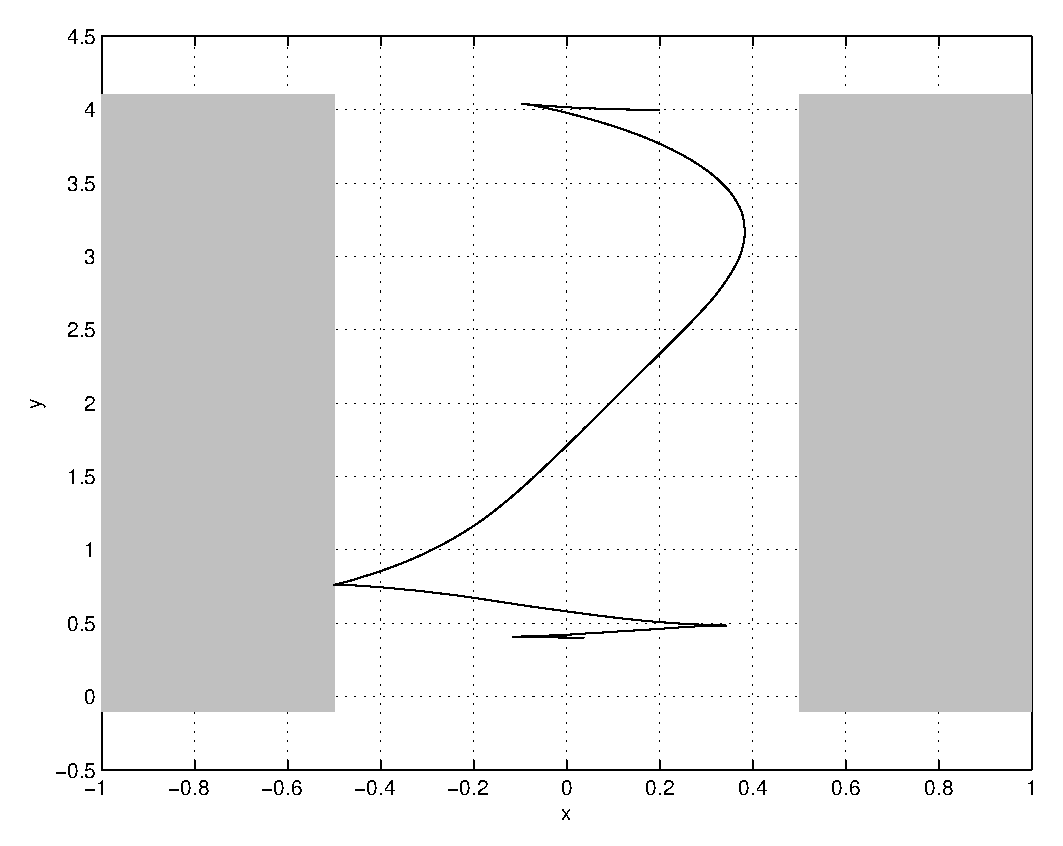
\includegraphics[width=\linewidth]{Figures/corridor1.eps}
    \caption{Trajectory in the $XY$ plane.}
    \label{fig:corridor1}
\end{figure}

Fig.~\ref{fig:corridor1} shows the trajectory of the MWR in the $XY$-plane. The grey areas are the walls of the corridor. It can be seen that there is a large steady-state offset in the $y$-state. As said in~\cite{essen01}, this is caused by a {\em dead-lock} situation the MPC algorithm should be able to recognize. On the contrary, this is not happen, probably because the nonlinear program solver is not able to generate persistently existing inputs for the uncontrollable system in {\em dead lock} situation~\cite{essen01}.

To eliminate this offset, a simple method is to use an additional penalty weight in the terminal state of the prediction horizon, thus forcing the states to converge to an acceptable solution. Hence, we have the following modified objective function:
\begin{multline*}
	\Phi(k) = \sum_{j=1}^{N-1}{\bf x}^T(k+j|k){\bf Q}{\bf x}(k+j|k) + \\ + {\bf u}^T(k+j-1|k){\bf R}{\bf u}(k+j-1|k)+ \Omega(k+N),
\end{multline*}
where $\Omega(k+N)$ is the terminal cost. Here we have used:
\begin{multline}\label{eqn:terminalcost}
	\Omega(k+N) = {\bf x}^T(k+N|k)100{\bf Q}{\bf x}(k+N|k) + \\ + {\bf u}^T(k+N|k){\bf R}{\bf u}(k+N|k)
\end{multline}
	
\begin{figure}[htbp]
	\centering
    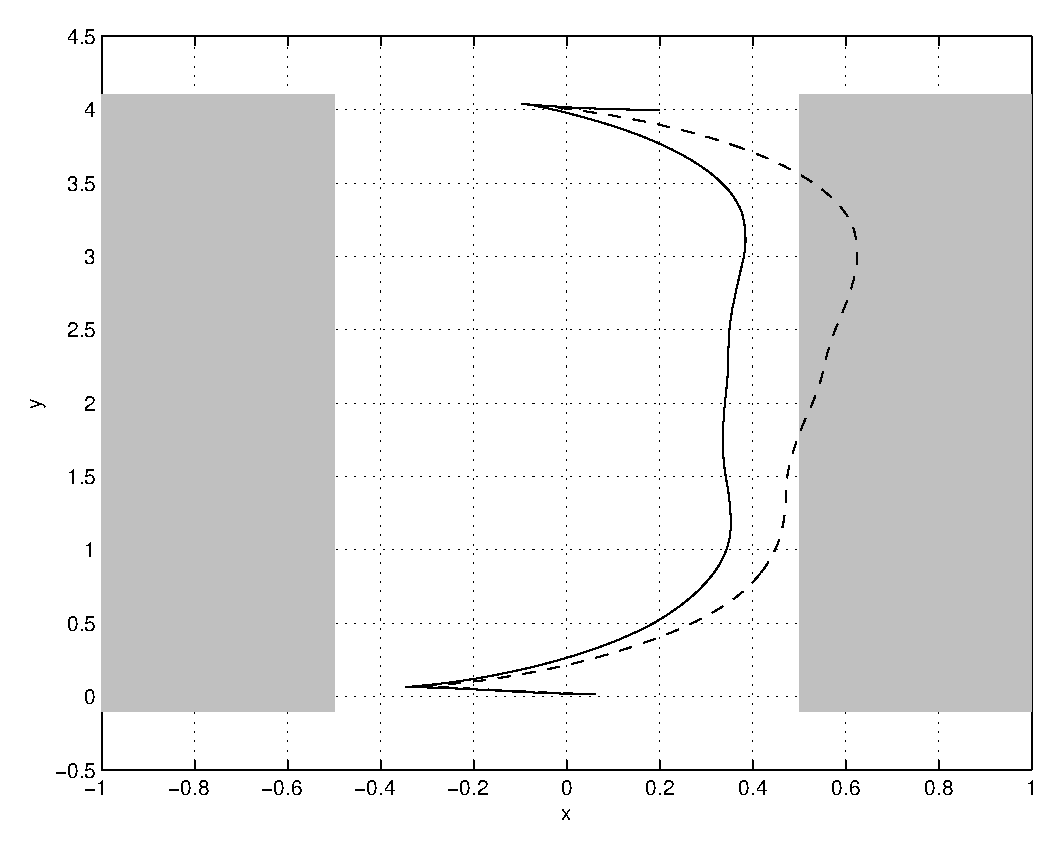
\includegraphics[width=\linewidth]{Figures/corridor2.eps}
    \caption{Trajectory in the $XY$ plane.}
    \label{fig:corridor2}
\end{figure}
\begin{figure}[htbp]
	\centering
    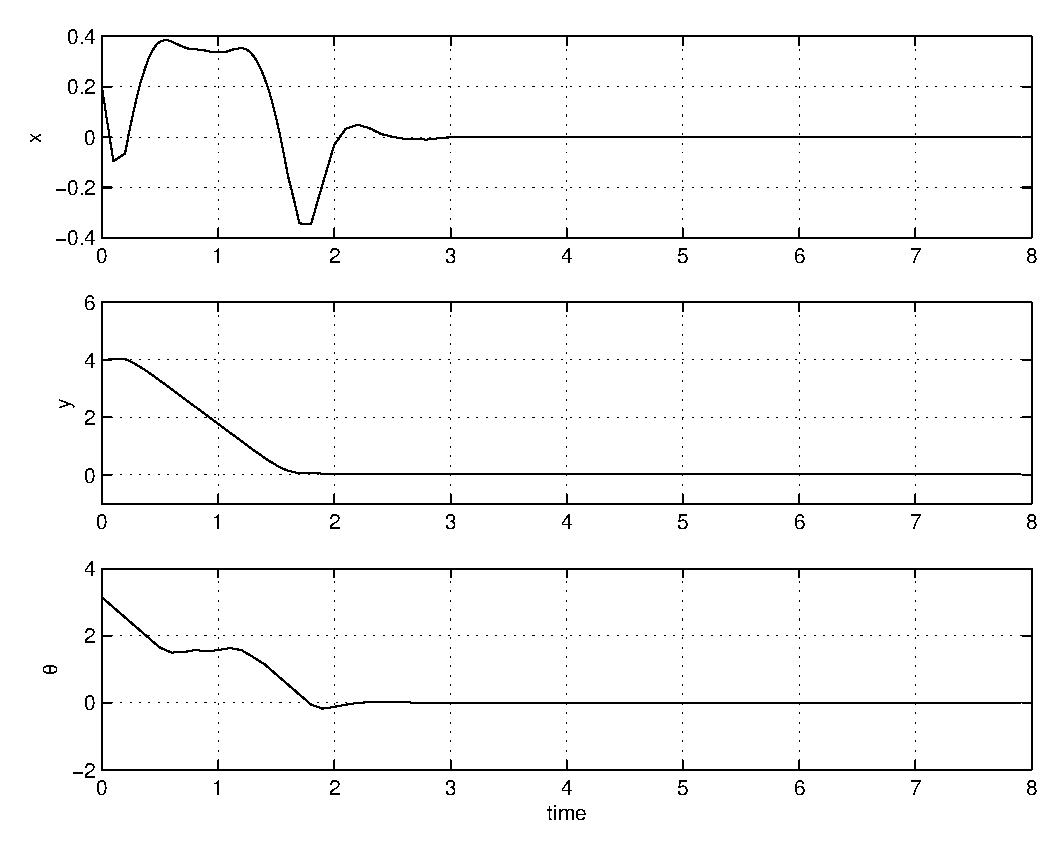
\includegraphics[width=\linewidth]{Figures/state2.eps}
    \caption{States $x$, $y$ and $\theta$.}
    \label{fig:state2}
\end{figure}
\begin{figure}[htbp]
	\centering
    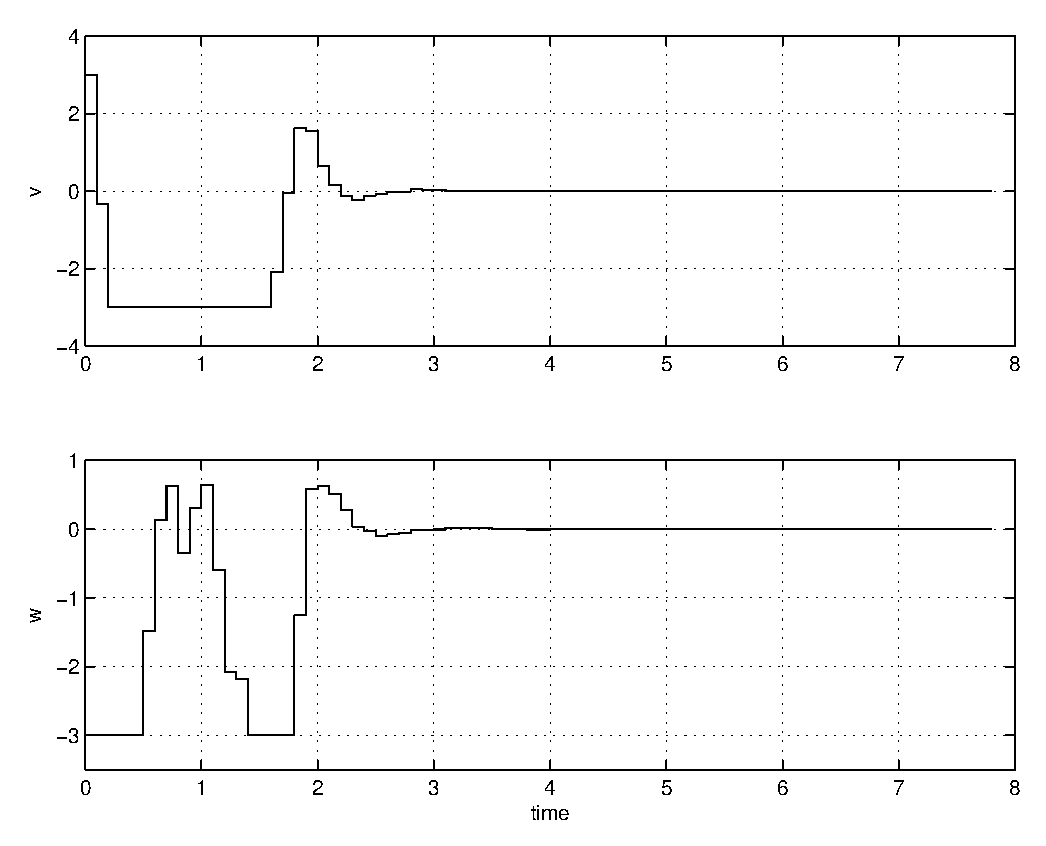
\includegraphics[width=\linewidth]{Figures/control2.eps}
    \caption{Control inputs $v$ and $w$.}
    \label{fig:control2}
\end{figure}
\begin{figure}[htbp]
	\centering
    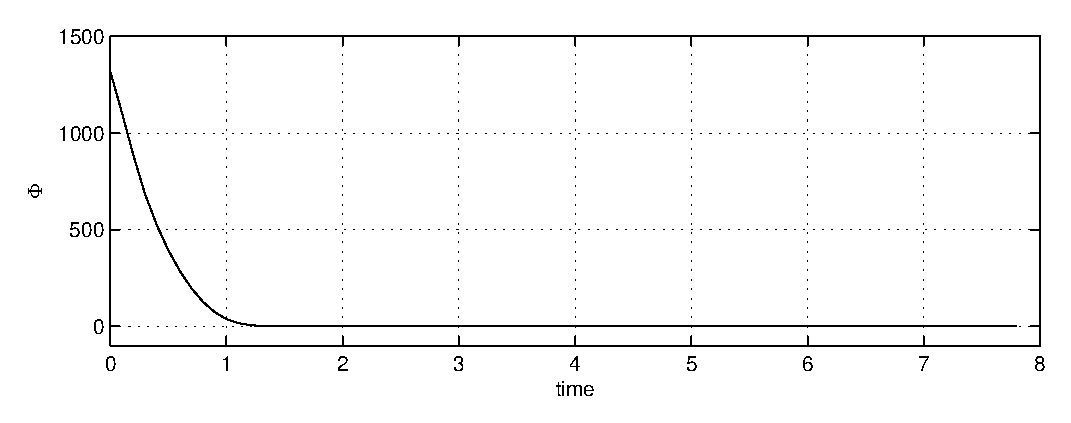
\includegraphics[width=\linewidth]{Figures/cost.eps}
    \caption{Objective function $\Phi$.}
    \label{fig:cost}
\end{figure}

Fig's.~\ref{fig:corridor2} and \ref{fig:state2} shows that, with the inclusion of the terminal cost~(\ref{eqn:terminalcost}), all states converge to the origin. The dashed line corresponds to the trajectory of the WMR when there are no state constraint. Since this trajectory invades the gray areas, the WMR would not be able to cross the corridor without crash in the walls.

Fig.~\ref{fig:control2} shows that the control inputs $v$ and $w$ are inside the limits imposed by the control constraints. Fig.~\ref{fig:cost} shows that the optimal value of the objective function converges to zero.

\section{Conclusion}
\label{sec:conclusions}

This paper presented an application of model predictive control to the problem of point stabilization of a nonholonomic wheeled mobile robot. Through an illustrative example -- the WMR crossing a corridor --, it was shown an important advantage of MPC: to handle input and state constraints. The obtained control signals were such that the constraints imposed on the control and state variables were respected. 

As shown above, the choice of MPC for the application given here is well justified by some advantages: the straightforward way in which state/input constraints can be handled; coordinate transformations to a chained or power form are not necessary; the MPC implicitly generates a time-varying control law, thus dealing with Brockett conditions.


\section*{Acknowledgments}

The authors gratefully acknowledge the financial support from CAPES.

% Equaliza as colunas da �ltima p�gina:
%\IEEEtriggeratref{6}

\bibliographystyle{IEEEtran}
\bibliography{yap}

\end{document}
